 \documentclass[12pt]{article}
\usepackage{amssymb,amsmath}
\usepackage[pdftex]{graphicx}
\usepackage{epsfig,subfigure}
\usepackage{epstopdf}
\usepackage{bm,url}
\DeclareGraphicsExtensions{.jpg,.pdf,.png,.eps,.ps}
\usepackage[usenames, dvipsnames]{color}
\usepackage{ulem}

\textheight = 522pt
\textwidth = 450pt
\oddsidemargin 0.0in

\newcommand{\Comment}[1]{\textcolor{Blue}{(Comment: #1)}}

\newcommand{\exec}{{Executive Team}}
\newcommand{\shorte}{{ET }}  %abbrev for \exec

%% Define a new 'leo' style for the package that will use a smaller font.
\makeatletter
\def\url@leostyle{%
  \@ifundefined{selectfont}{\def\UrlFont{\sf}}{\def\UrlFont{\small\ttfamily}}}
\makeatother
%% Now actually use the newly defined style.
\urlstyle{leo}

\begin{document}

\title{CMB-S4 Collaboration Bylaws}
\maketitle


\tableofcontents

%\Comment{ADD COMMENTS WITH $\backslash$Comment\{ \} }

\newpage


%\section{Collaboration Governance Objectives/Preamble}
\section{Preamble}

The CMB-S4 collaboration will carry out a CMB science program including the design and construction of the future experiment that is intended to be the definitive ground-based CMB program. CMB-S4 will deliver a highly constraining data set with which any model for the origin of the primordial fluctuations---be it inflation or an alternative theory---and their evolution to the structure seen in the Universe today must be consistent. This document outlines the CMB-S4 collaboration governance and organization of scientific activities.

\subsection{Collaboration Governance Objectives}
 The collaboration will adhere to the following principles:

\begin{itemize}
\item The Collaboration will be organized based on models used in other successful  large DOE and NSF-supported experiments.  %Cosmic Frontier 

\item The Collaboration will strive to maximize the scientific return of the experiment, producing high-quality science in a timely manner and promoting full utilization of the data through public data releases after a suitable proprietary period.

\item The organizational structure of the collaboration should enable broad representation of members, and encourage consensus in decision making. %while fostering 

\item   All members of the collaboration will be expected to contribute to the success of the project through work on one or more areas of necessary infrastructure. The organizational structure should incentivize collaboration members to contribute to the execution of the project including work on hardware, software, testing, commissioning, operations, common science infrastructure, documentation and publications.  

%\item All members of the collaboration will be expected to contribute to the success of the project through work on one or more areas of necessary infrastructure.

\item Towards this end, the collaboration should provide appropriate credit to data analysts, hardware and/or software builders; provide leadership opportunities and other opportunities to promote career advancement; motivate people to work together towards common goals to complete the key project deliverables; and provide a healthy collaboration culture that establishes standards for behavior consistent with high ethical standards.

\end{itemize}


\subsection{Definitions}

Throughout this document,  a ``supermajority vote" is defined as a result with more than two-thirds of the votes received in favor of the motion.   A ``majority vote" requires only half the votes received.   Two-thirds of eligible voters must cast votes (including abstentions) for a vote to be valid.    A ``quorum" for a meeting is defined as the presence of a majority of a body's members.   For collaboration-wide votes, a ``Voting Member" is  defined as a Senior Member or a Postdoctoral Member (see \S\ref{sec:memberrights}). ``Ex officio" members of a governance body are those whose membership is due to their roles elsewhere in the Collaboration.  For example, the Science Council chairs (\S\ref{sec:SC}) are ex officio members of the Executive Team (\S\ref{sec:exec}).  

 %The presence of a simple majority of a body's members constitutes quorum for a meeting, and two-thirds of a body must be present for a vote to be valid.

%Add definition of �ex officio� membership as membership by virtue of having another role, so that the Science Council chairs are ex officio members of the ET,  and when a new chair is elected, the old chair rolls off the ET. 



\section{Overall Structure}
The Governance Structure of the CMB-S4 collaboration consists of three bodies: a Governing Board (GB), an \exec \ (\shorte), and two equal co-spokespersons (SP). 
Under each of these bodies a number of councils, committees, and working groups are established to ensure timely and efficient conduction of the duties assigned to each body. The overall scope, selection of, and interplay between each of these governing entities is described in the remainder of this document. 


\begin{figure}[h!]
\begin{center}
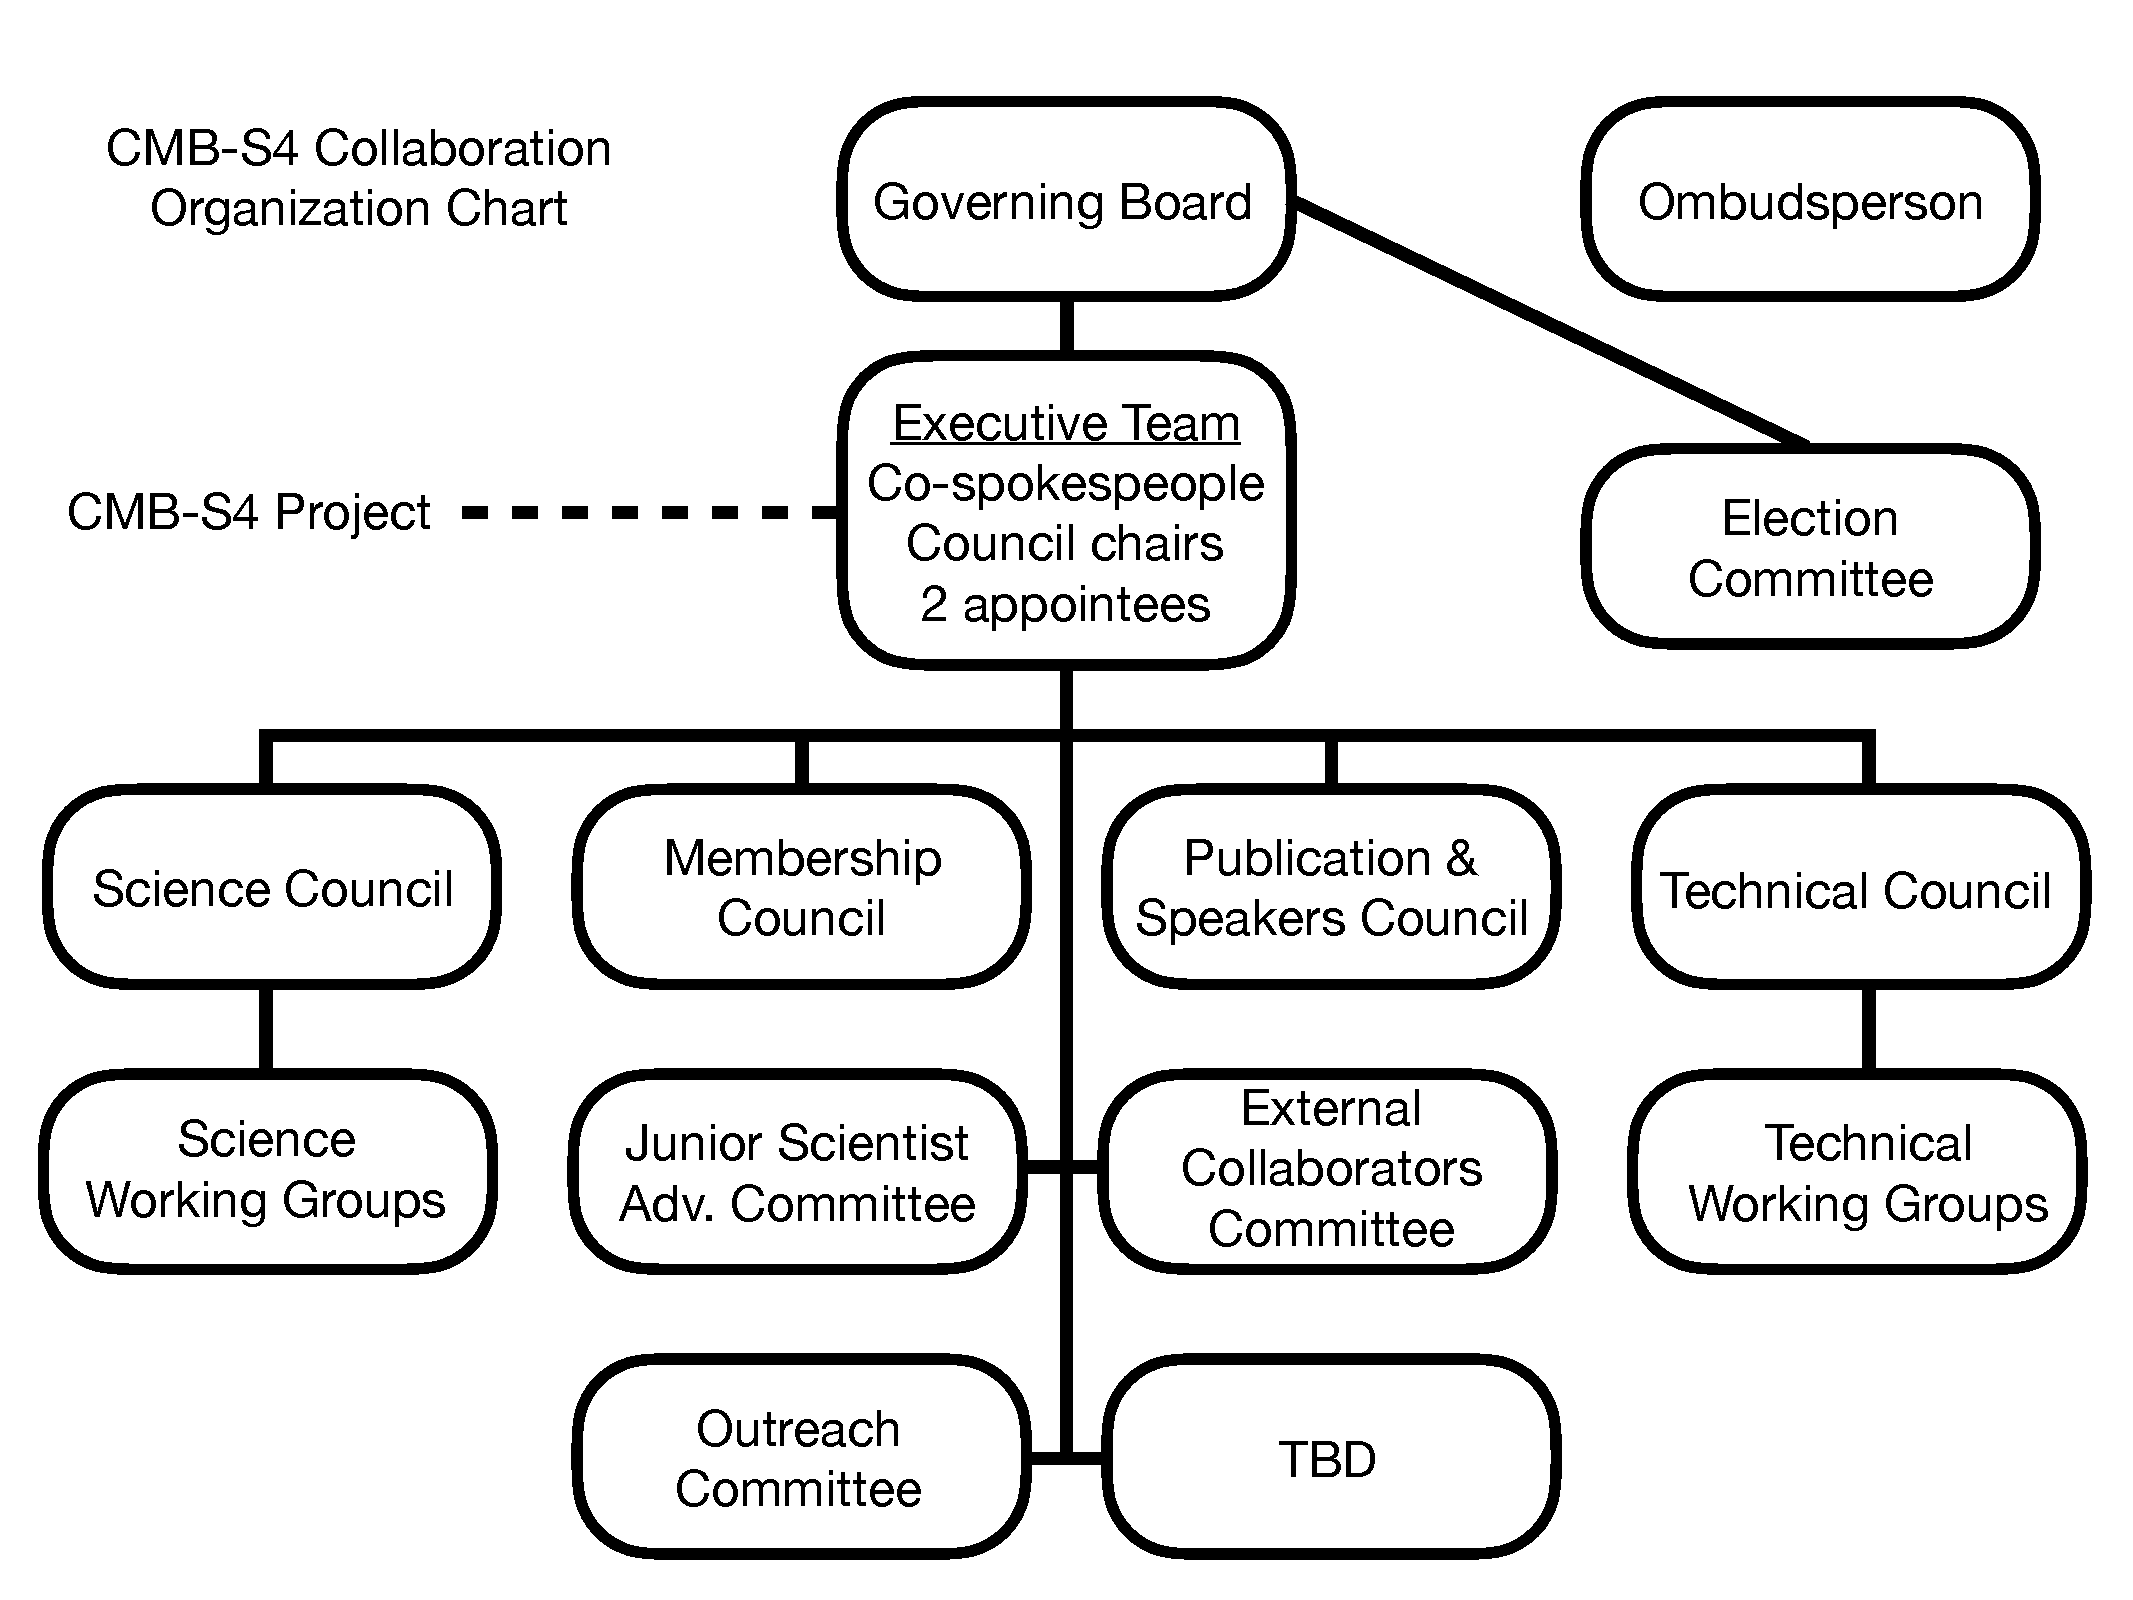
\includegraphics[width=6.5in]{CMB-S4_Org_chart_+_details_v6.pdf}
\end{center}
\caption{CMB-S4 Collaboration Organizational Chart version 4}
\label{fig:org_chart}
\end{figure}

\section{Governing Board}

The Governing Board, a body whose composition is designed to be representative of the membership of the collaboration as a whole, is the ultimate policy forming body of the CMB-S4 collaboration. 

\subsection{Scope}
The Governing Board has two main roles: to facilitate discussion of collaboration-wide issues---especially those that concern the self-governance of CMB-S4 Collaboration as a whole---and to provide oversight of both the \exec \ and the co-spokepersons.
Governing Board activities include, but are not limited to: 

\begin{itemize}
\item Approval and revision of Collaboration Bylaws; amendment of the Bylaws requires a super-majority of the GB. This excludes any Bylaws that directly pertain the power, scope, election, etc. of the GB, which will be discussed in Section \ref{subsec:amend}.


\item Charging the co-spokespersons to carry out specific duties for the collaboration, including, but not limited to, collaboration reviews, committee, and board reviews. 

\item Charging the co-spokespersons with preparation of a yearly plan for the collaboration and the ratification of this plan. 

\item Oversight of the activities of the co-spokespersons. The GB may require a detailed verbal, or written report from the co-spokespersons on any action. 

\item Membership conflicts/issues, such as the removal of members and institutions from the collaboration. Removal of a member requires approval by a super-majority of the GB.

\item Organization of elections for Spokespersons, GB members, \shorte \ members, and other elected collaboration officials.

%\item Oversight of various collaboration sub-committees and councils including, but not
%limited to: Elections, Membership, Publications, Science Council, Education and
%Public Outreach, and the Junior Scientist Advancement Committee, through reports
%from both the co-spokespersons and \exec \ as well as other required duties spelled out in these Bylaws. \textcolor{red}{Keep or remove this? (E.g., Reading pubs section - the GB ratifies pub policy changes so it seems it would be good to clearly state that the GB might interact with these bodies}

\item Approval of additional long-standing sub-committees as required. This may include promotion of short term sub-committees established by the co-spokespersons to long-term status. 

\item \textcolor{red}{Ratification of changes to the Speakers/Publications Policy.}

\end{itemize}

\textit{Any powers not explicitly assigned to a different governing body in these bylaws reside in the Governing Board}. 

\subsection{Board Representation}
The GB will be composed of 19 members. 
To ensure that the board is truly ``\textbf{representative}'' of the collaboration, prior to the election the GB---or the ICCC for first election---will define various categories of representation it is deemed important to include on the GB (possibly including e.g., ``Tenure Track" early career scientists,  historically underrepresented groups, partner countries with significant membership, members of small institutions, etc). Both the GB and spokespersons---or the ICCC for first election---should particularly encourage suitable candidates in each of these categories to self-nominate for board membership.

The length of a term of service for a Governing Board member is two years; members are allowed to serve at most two terms consecutively.
Further details on the election of GB members are provided in Section \ref{sec:elections}.


\subsection{Governing Board Chair}

The GB chair is responsible for scheduling GB meetings, distributing the agendas, chairing the meetings, and distributing the minutes. The GB secretary can be delegated to take and distribute the minutes. 

\subsection{Election of the Governing Board Chair}
The GB chair will be elected from amongst the board members. 
Every year, starting with the inception of the GB, the chair of the GB is elected from the GB membership to serve a one-year term. GB members nominate candidates by email and then vote by email, with the votes in both cases tabulated in secret by a third party agreed upon by the GB at large. The candidate with the most votes becomes the GB chair. In case of a tie, a runoff election is held. In case of a tie in the final runoff, the chair will recuse him/herself from the vote to resolve the tie, but otherwise he/she is eligible to vote in the election. The secretary of the GB, should one be used, is chosen informally by the chairman of the GB to serve during his or her term. \Comment{1 year chair term to deal with staggered board elections}


\subsection{Governing Board Meetings}
\textit{The first chaired Governing Board will establish rules for its meetings}. This first meeting will be held no later than 2 months after the selection of the board.  It is expected that the board will meet no less than every two months to ensure adequate attention to its duties. Such meetings will likely occur in closed session at every CMB-S4 collaboration meeting and in meetings held by telephone or video conference. Special meetings can be called on the initiative of the GB chair or at the request a GB representative. Each meeting requires a quorum to conduct official GB business.
GB votes can be held by email. Minutes of the GB meetings are distributed to the full CMB S4-collaboration by the GB chair or GB secretary. These minutes must include meeting attendance and the records of the votes cast by all GB members. It is the expectation that GB members participate in the majority of meetings. If a GB member fails to participate (via meeting attendance or email) in $>50\%$ of GB meetings in a year, their seat will be open to election during the following cycle and they will be barred from the board for a two year term.  

\subsection{Election and Voting Commission}
The GB appoints the chair and two additional members of the Election and Voting Commission (EVC).  The EVC is charged with conducting elections as spelled out in \S\ref{sec:elections}. The EVC acts \textbf{independently} of the GB, but any points of substantive disagreement amongst the members should be referred back to the GB.  Commission members serve two-year terms ordinarily.  However, the GB may choose to extend the first term of the chair to  three years, to allow staggering of the membership for improved continuity between commissions.   Commission members may be removed with a supermajority vote of the GB.
 % , with the exception of the chair who will serve a three-year term at the start of the collaboration (the chair position is a 2 year term thereafter) to enable a continuity between commissions. There are no term limits for this commission. 
\subsection{Amendments to the Governing Board Bylaws by the Governing Board} \label{subsec:amend}
Any amendments made by the Governing Board that pertain to its own election,governance, and scope must be ratified by a majority of the voting members of the collaboration.


\section{Co-Spokespersons}
\label{sec:spokes}

\subsection{Scope}

The	scientific leadership of the CMB-S4 collaboration resides with two equal co-spokespersons.			
Each spokesperson participates actively in the management of all aspects of the	collaboration and, as the executive officials of the Collaboration are responsible for its day-to-day management. 
To carry out their duties, the spokespersons are expected to solicit advice from the collaboration at large, the Governing Board, and the	
\exec \ on scientific, technical, management, financial, and leadership issues.  
Duties include, but are not limited to the following: 
\begin{itemize}
\item Serving as the primary contacts with a  host laboratory/institution (if one exists), the funding agencies, scientific organizations, and the press. Reports on such activities will be provided on a semi-annual basis or by request to the Governing Board.
\item Assuring public dissemination of scientific results. 
\item Creation of short-term ad hoc committees for the purpose of such tasks as creation of review materials, white papers, exploration of new partnerships, etc.
\item Organizing and running collaboration meetings. 
\item The co-spokespersons may appoint up to two members of the \exec. This appointment flexibility will enable the SPs to obtain expert advice on an as-needed, short-term basis for matters including (but not limited to) technical and managerial topics that may be outside the expertise of extant collaboration members. Such appointees will be approved by the GB, 
and may be removed from the board at the co-spokespersons' discretion. Appointments are limited to 2 years, but may be renewed with approval of the GB. 
\item Carrying out other duties as charged to them by the Governing Board.


\end{itemize}
Additionally,the co-spokespersons are ex-officio, non-voting members of the Governing Board.  \textit{The Governing Board, via super-majority vote, may amend these duties.} 
Spokespersons are elected to two-year terms. \textbf{There are no term limits specified at this time, but term limits of 2 terms are to be imposed once CMB-S4 is more established as a project}. The election process is detailed below in Section \ref{sec:elections}. 

\subsection{Removal of a Spokesperson}

The GB can remove a spokesperson by a secret ballot, requiring approval by a super-majority of the GB. A two-week collaboration-wide notice is required for a vote for removal and such a vote will be taken if at least half the GB members support such a proposal to the chair. After the vote is taken the record of the vote (e.g., who voted and how) will be made available to the collaboration. In the event of a removal, the open position(s) will be filled following the procedures in these bylaws.


\section{\exec}
\label{sec:exec}

\subsection{Scope}

The \exec \ (\shorte) is an elected and appointed board that consists of up to 10 members: the co-spokespersons and both the elected chair and deputy of the Science Council, the  chair and deputy of the Technical Council, the chair of the Membership Council, the chair of the Publication and Speakers council, and up to two appointed members. This Board is the agile decision making body in the collaboration with the ability to address the day-to-day collaboration issues. 

The \exec \ has three main roles:
\begin{itemize}
\item to facilitate the flow of information to the co-spokespersons from the collaboration and vice versa.

\item to provide leadership on scientific, membership, financial, and organizational decisions and issues. The decisions will ultimately be made by the co-spokespersons, but will be discussed and reasoned through the \exec.  However, any two \shorte members may call for a vote on any topic, and if $\geq 50\%$ of the board is in disagreement with proposed activities of the Spokesperson, the issue is referred to the Governing Board for further discussion. 

\item to aid the co-spokespersons in being the collaboration liaison to the project. In the event that the co-spokespersons do not agree on a particular topic, the \shorte will hold a vote requiring only a majority.

\end{itemize}

Elected \exec \ members serve two year terms with elections governed as described in Section \ref{sec:elections}. The appointment of up to two \shorte members by the co-spokespersons is described in Section \ref{sec:spokes}. 

\subsection{Removal of an \exec \ member}

As with a co-spokesperson, the GB can remove an \shorte member by a vote, requiring approval by a super-majority of the GB.  A two-week collaboration wide notice is required for a vote for removal and such a vote will be taken if at least half the GB members support such a proposal to the chair. After the vote is taken the record of the vote (e.g., who voted and how) will be made available to the collaboration. In the event of a removal, the open position(s) will be filled following the procedures in these bylaws.

\subsection{\exec \ Meetings}

The co-spokespersons will chair the meetings, provide the agenda, and establish rules for these meetings. This first meeting will be held no later than 2 weeks after the election of co-spokespersons and the committee chairs. It is expected that the board will meet no less than twice a month to ensure adequate attention to its duties. Meetings can be called on the initiative of a co-spokesperson or at the request an \shorte member provided that a co-spokesperson agrees. A summary of the \shorte meetings will be distributed to the collaboration. Each meeting requires a quorum to conduct official ET business.  It is the expectation that \shorte members participate in the majority of meetings; \shorte members who fail to participate via active live attendance or email in $\geq 50\%$ of meetings will be replaced in the nearest election cycle and barred from the \shorte for a two year term.  


\section{Elections}\label{sec:elections}
All elected positions of the major bodies in the CMB S4 Collaboration serve two year terms. Elections for each of these bodies will be arranged so that $\sim 50\%$ of the members in each body will be up for election each year. In this section of the bylaws the process and timing for each major election is described.  As there are restrictions placed on the overlap of elected officials between various governing bodies elections are timed to provide collaboration members with multiple opportunities to participate in collaboration governance. 
Figure \ref{fig:elect_cycle} displays schematically the timing of the election cycles described below.  

In a given election year the ordering shall proceed as follows: first elections will be held for co-spokesperson. Next elections will be held (if required by term completion) for science council chair or deputy chair, chair of the membership council and chair of the publication and speakers council. A third election will be held for Governing Board members. 
Elections for positions outside the top levels of major bodies may occur when required as such officials are not prohibited from serving other elected roles. Each election is managed by the Election Committee established and overseen by the Governing board. The ICCC must establish this committee prior to the formation of the CMB-S4 collaboration. 


\begin{figure}[h!]
\begin{center}
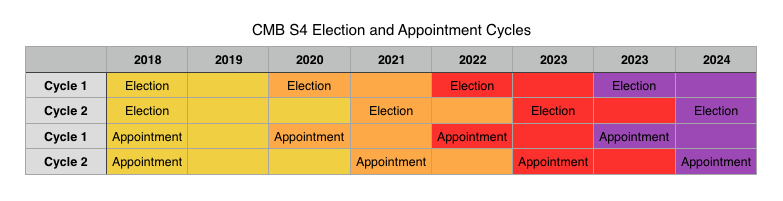
\includegraphics[width=6.5in]{Election_cycle.png}
\end{center}
\caption{CMB-S4 Election and appointment cycles. Note that for the cycle 1 elections 50\% of a given body will serve a 3 year term to enable staggered elections/appointments in future cycles.}
\label{fig:elect_cycle}
\end{figure}

\subsection{Elections of a Co-Spokesperson}

Co-Spokespersons are elected to two-year terms. All senior collaboration members (as defined in the membership section below) are allowed to run for these positions.  Normal co-spokesperson elections will be timed such that a slate of nominees can be presented at the GB meeting closest to January 1 each year. The Co-Spokesperson elections will occur prior to elections of the Governing board. As a Co-spokesperson can not be a voting member of the GB, if a voting member of the GB is elected to a co-Spokesperson position they must resign their GB seat prior to the start of Co-Spokesperson term and this vacancy will be filled in the next GB election. 

Prior to the election, qualified electors---as specified in the membership section below---are asked to nominate individuals by the Election Committee. Each elector may nominate one candidate and self-nominations will be accepted. A minimum of two nominations are required for a nominee to be eligible to appear on the slate of election candidates. After a nomination period, the election committee  will consult with the nominees to ascertain their willingness to stand for the election.

If no candidate agrees to stand for election, the terminating co-spokesperson will continue to serve for six months, after which a special election will be held. The term of the individual elected in a special election will be reduced by the amount needed to cause the sum of his/her term and the additional months served by the terminating co-spokesperson to equal two years.

The election is held through an on-line poll, with votes submitted by qualified electors. The election committee will preside over the election results. Each candidate will provide a Candidate Statement to the committee, which will collect these documents and make them available to the collaboration via the CMB-S4 internal web page prior to the balloting. The election committee, in consultation with the GB (or ICCC), determines the detailed timing of the balloting and determines procedures for dealing with any election situations not anticipated in the bylaws. Each qualified elector votes for a single candidate for each vacant position; in the first election, in which two co-spokespersons will be selected, collaboration members may vote for two candidates. 

The election committee checks the ballots against the list of qualified voters and tallies the votes. For the first election, the two candidates with the most votes will be elected spokesperson, with the candidate with the highest vote total selected for a 3 year term to enable offset elections of future spokespersons.  In the event of a tie, a runoff election will be held between the two candidates that have the same number of votes. The elected candidates will take office when the election committee announces the results of the election to the collaboration via email. 

\subsection{\exec}
Following conclusion of the Spokesperson election, elections for various elected positions on the \exec \ will be held during the final year of each position's two year cycle. The process for these elections proceeds in an identical fashion as to the Spokesperson election. 

\subsection{Governing Board Elections }

Every year, following completion of the co-spokesperson election and any required \exec \ elections, the Election Committee then carries out elections for seats on the Governing board whose term is expiring in less than 12 months. The election committee first solicits self-nominations for Governing Board membership and candidate information is then circulated to qualified electors as defined in the membership section of these bylaws. Electors vote via email, with the votes tabulated by the Election Committee members not standing for election (or, in cases where the whole committee is conflicted, by a third party appointed by the Co-Spokespersons). During the election, each elector may vote for 50\% of the total number of board members. 


\subsubsection{The First Election of the Governing Board}
For the first election, the top 10  vote-receiving candidates are automatically selected for the board. If representation requirements outlined above are unfulfilled by the elected candidates the remaining open seats are filled via total votes cast until seats are needed to ensure representation requirements are met. At this time the outgoing ICCC is empowered to fill the open seats to meet these requirements. 
To enable offset elections (to ensure an element of continuity in the GB), 50\% of the first GB members will serve 3 year terms as determined by random draw. 

\subsubsection{Election of the Governing Board after the establishment of the Collaboration}
 After the collaboration is established, the GB is to amend these bylaws to establish whether to have separate votes for each category of representation or to continue with a mixed election/appointed governing board model. It is the expectation that the GB be moved to a fully elected body as the collaboration matures. 

\subsection{All Other Elected Positions}
For other elected Collaboration roles, the Election Committee is charged with establishing election rules and conducting these elections. Note that the committee \textbf{can not} make voting requirements more restrictive than those for the main body elections. Elected  roles in additional positions are limited to at most 2 year terms. 


\section{Science Council}
\label{sec:SC}

The Science Council is one of the major bodies established by the Governing board and overseen by the Spokespersons. It is charged to coordinate---in consultation with the co-spokespersons---the key scientific objectives of the CMB S4 collaboration. The Science council chairs are also members of the \exec. \textcolor{red}{The Science Council is responsible for maintaining a list of ``Key'' Science Topics as discussed in Section (PUB SECTION)}. 

The Council is composed of an overall chair and deputy-chair elected by the full S4 collaboration, as well as the co-coordinators of the various scientific working groups. These working groups are to be formally established by the Co-spokespersons,
but will likely include groups similar to those established for the first CMB S4 science book, but not limited to the science book. 

Each working group will have two co-coordinators who each serve for two year terms with the exception of one initial coordinator who will serve for a 3 year term to enable staggered appointments in the future.  The Science Council chairs will solicit self-nominations for these co-coordinators positions. The SP will appoint coordinators with the advice of the Science Council chairs while considering the distribution of early and late career members when making these appointments. Coordinators will ordinarily not serve back-to-back terms.


\section{Technical Council}
The Technical Council (TC) is a temporary major body established by the Governing Board and overseen by the Co-spokespersons. Prior to the formation of the Project, the TC is charged to coordinate---in consultation with the Co-spokespersons---the technical aspects needed to meet the scientific objectives of the CMB S4 collaboration. The TC chairs are also members of the \exec. 

The Council is led by an overall chair and deputy-chair appointed by the Co-spokespersons and ratified by the Governing Board.  The co-leads of the various technical working groups are all members of the TC.  These working groups are to be formally established by the Co-spokespersons.   

Each working group will have two co-coordinators who each serve for two year terms with the exception of one initial coordinator who will serve for a three year term to enable staggered appointments in the future, as needed.  The Technical Council chairs will solicit self-nominations for these co-coordinator positions. The Co-spokespersons will appoint coordinators with the advice of the Technical Council chairs while considering the distribution of early and late career members when making these appointments.

We anticipate the role of and/or the need for the Technical Council will be readdressed in these Bylaws when a Project is formed.

\section{Membership Council}

The Membership Council (MC) consists of 7 people including a council chair. The chair is elected following the election cycle of the collaboration with  2 year terms, and is limited to 2 consecutive terms with 1 year off required before standing again. The 6 remaining members are appointed by the \shorte with the same term limits. If a council member leaves before their term is completed they may be replaced by the co-spokespersons with the ratification of the \shorte until the next election cycle occurs. MC members can be removed by a super majority of the GB at any time.  


The appointed members should represent the overall collaboration, and there should be at least 2 members from the technical working groups and 2 members from the analysis working groups in the overall council. This balance may be amended as the scientific needs of the collaboration evolve. \Comment{This leaves two spots to encompass people who might not fall neatly into either group.}

\section{CMB-S4 Collaboration Membership Policy}

The CMB-S4 collaboration consists of Ph.D. scientists, engineers, Ph.D. thesis students %undergraduate students, 
and others who contribute significantly to the CMB-S4 program. Membership conveys certain rights as described below, but comes with the obligation of an ongoing commitment of a substantial fraction of members' research time to the CMB-S4 program.

\vspace{0.2in}
\noindent


\subsection{Membership Council}

The duties of the Membership Council are to review and evaluate membership applications, review annual activity reports, and recommend changes in membership status. 

\subsection{Membership Types}

\begin{itemize}

\item {\bf Senior Member:} A Senior Member of the collaboration is a member who has a permanent appointment or an appointment, that under normal circumstances can be expected to be renewed indefinitely.   This includes tenure-track appointments at universities and their equivalents elsewhere.  

\item {\bf Postdoctoral Member:} A postdoc working with a Senior Member at their institution can be designated as a Postdoctoral Member by that Senior Member.  Postdocs that reside at an institution where there is no Senior Member can apply to become a Postdoctoral Member and have their application evaluated by the Membership Council on a case-by-case basis. 

\item {\bf Student Member:} A graduate student working with a Senior Member at their institution can be designated as a Student Member by that Senior Member.  We do not anticipate granting membership to students who are not supervised by a Senior Member.

\item {\bf Provisional Member:}  A Provisional Member is a potential senior member who has not yet been approved for senior member status.  This is intended to be a temporary status allowing the member to demonstrate constructive engagement with the collaboration at a level that qualifies them for Senior Membership.

\item {\bf Legacy Member:}  A Legacy Member is a former member who contributed in a key manner to the project infrastructure, but is no longer engaged with the collaboration and is therefore no longer a member.  This status is intended to convey authorship rights to such former members, and to bypass the normal membership procedures should they wish to re-engage with the collaboration.

\end{itemize}



\subsection{Membership Rights}\label{sec:memberrights}

Herein, ``members'' refers to Senior, Postdoctoral, Student and Provisional members (but not Legacy Members) unless otherwise qualified.  

\begin{itemize}

\item Senior and Postdoctoral Members are Voting Members.  Voting Members  have the right to vote to ratify Bylaws and amendments to Bylaws, and vote in elections for Spokespersons, Governance Board representatives, and othe elected positions including the chairs of the Science, Membership, and Publication and Speakers Councils.  %vote for representation on the Governing Board.  

\item Members have full data access, including during the proprietary period for data that are eventually released.

\item Members (including Legacy Members) have the right to be listed as a co-author on CMB-S4 publications as specified in the Publication Policy.

\item Members have access to computational resources designated for CMB-S4, according to the policies of the relevant computational resources working group.

\end{itemize}

\subsection{Membership Requirements}
\begin{itemize}

\item Members must commit effort to approved infrastructure tasks, which can include, for example, designing, building, and testing software, hardware, or simulations, as well as management. 

\end{itemize}

\subsection{Membership Application and Approval Process}
After the CMB-S4 collaboration is formed with a first set of initial members (see Section \ref{sec:initmembership}), the process for membership to CMB-S4 will be as specified below.

\begin{itemize}

\item Potential Senior Members will apply for Provisonal Membership via a written application where they specify their proposed work on CMB-S4. 

\item Independent postdocs not co-located with a Senior Member can apply for Postdoctoral Membership and have their application reviewed on a case-by-case basis. 

\item Postdoctoral members can apply for ``Intended Senior Membership Status", which would convey that the postdoc will have Senior Membership status when moving to a permanent appointment or an appointment that, under normal circumstances, can be expected to be renewed indefinitely.  The Membership Council will decide the requirements for achieving this status, the achievement of which grants Senior Membership at the new institution.

\item Applications are reviewed by the Membership Council. The Membership Council recommends membership to the Governing Board.  The Governing Board approves membership.

\end{itemize}

\subsection{Initial Membership}
\label{sec:initmembership}
The CMB-S4 collaboration will initially consist of members who have satisfied the following criteria:

\begin{itemize}
\item Attended at least two CMB-S4 collaboration meetings, and 

\item Voted on the governance bylaws.
\end{itemize}

Within the first year of the Collaboration's establishment, prospective members can be granted membership by successfully petitioning the Membership Council despite not satisfying the above criteria.  The Membership Council may approve such applications during the first year without action by the Governing Board.  

\subsection{Membership Review and Changes in Status}
\begin{itemize} 

\item Each Senior Member, and each independent postdoc not co-located with a Senior Member, will submit an annual activity report to the Membershp Council.  Senior members can discuss activities of their supervisees (e.g. postdocs and students) in their report. The Membership Council will review those reports, consulting with collaboration members and working group leaders as appropriate.

\item Provisional members will submit a annual activity report to the Membership Council, which will review the report and determine whether the provisional member should be promoted to a Senior Member status, continue as a Provisional Member, or have their membership revoked.  Provisional Membership is intended to be a temporary status.

\item Members leaving the collaboration may be granted Legacy Membership upon review by the Membership Council and approval by the Govering Board.

\item If the effort of any member over the previous year seems lacking, the Membership Council will bring this to the attention of the Co-spokepersons and the Governing Board.  This can also be done at any time, should the Membership Council deem the actions of a member to have been egregious and detrimental to CMB-S4.

\item The Governing Board has the authority to grant or terminate all forms of membership.

\item When a person's membership in the collaboration is terminated, they will no longer have access to the CMB-S4 document and database repository, internal forums, computing resources and data.  Authorship rights will continue, or not, as prescribed in the Publication Policy bylaws.


\end{itemize}

\subsection{Procedure to Change Membership Policies}

The Governing Board may change Membership policies by a 2/3 majority vote of voting members.

%\section{Collaboration and Institution Membership}

\subsection{Requirements for Admission}

The CMB-S4 collaboration consists of Ph.D.\ scientists, engineers, Ph.D. thesis students, undergraduate students, and others who contribute significantly to the CMB-S4 program. A rough guideline is that all collaborators should devote a substantial fraction of their research time to the CMB-S4 program over a period of several years.
Visiting scientists and engineers (henceforth visitors), such as faculty members on sabbatical at a CMB- S4-affiliated institution, may also be admitted to the collaboration as short-term members, provided they devote a substantial portion of their research time to the collaboration.

The process of admission to the collaboration shall accord with the membership rules applicable to their degree of seniority. A senior member of the collaboration is a member from a collaborating institution who has a permanent appointment or an appointment that under normal circumstances can be expected to be renewed indefinitely. All other members of the collaboration are regular members. Senior members are admitted to the collaboration individually. Regular members are selected by their institutions. The only distinction between senior and regular members is the method by which they are admitted to the collaboration.
Senior members are admitted to the collaboration in one of four ways:
\begin{enumerate}
\item by being on the qualified elector list at the time of the initial spokesperson election,
\item by being on the approved list of senior members when their institution was admitted to the collaboration,
\item by being a regular member of the collaboration and receiving a position at any collaborating institution that would qualify him or her for senior membership status,
and
\item by individual application.
\end{enumerate}
A senior physicist at a collaborating institution who is not a member of the collaboration, and who wishes to join the collaboration, applies for membership in the same way as a new institution, as provided in Section 6. This procedure applies as well to visiting senior personnel applying for short-term membership.

The membership list is distinct from the author list described in Section \ref{sec:pub}.

\section{Admitting New Institutions}

To apply for membership in the CMB-S4 collaboration, representatives from the institution should first confer with the spokesperson. The representatives then submit a written proposal to the IB chair at least two weeks prior to the meeting of the IB at a regularly scheduled collaboration meeting. The IB chair circulates the proposal to IB members prior to the meeting and puts consideration of the application on the meeting agenda.

The proposal should describe the contributions that the prospective institution proposes to make to the collaboration and should include a list of the proposed senior members from the institution. The spokesperson will present the proposal to the collaboration by the prospective institution. This presentation should occur prior to the IB meeting held during the same collaboration meeting. The IB may: (1) approve the proposal and formally admit the institution to the collaboration at that meeting, (2) request further written clarifications to be considered at the next collaboration meeting, or (3) reject the proposal. The IB will attempt to make decisions on admission of new institutions by consensus. If consensus is not possible, a vote by secret ballot will be taken on admission. Admission will require a favorable vote by a super-majority of IB members present and voting.

\section{Removal of Collaborators and Institutions, Updating Membership and Leaving an Institution}

\subsection{Removal of Collaborators and Institutions}

Annually the IB Chair, in consultation with the spokesperson, will identify inactive institutions, using the criterion that an active institution has performed a reasonable amount of work on CMB-S4 within the previous twelve months. The IB may remove inactive institutions from the collaboration by a super- majority vote.

Individual collaborators who have not performed a reasonable amount of work on CMB-S4 for a period of at least twelve months, or whose behavior has been egregious and detrimental to CMB-S4, may be removed from the collaboration at an IB meeting by a super-majority vote of the IB members present and voting.

\subsection{Updating CMB-S4 Membership Rolls}

Each CMB-S4 IB member will be responsible for updating and verifying the collaboration membership list for his/her institution. A yearly questionnaire will be distributed by the IB chair to each institution to help keep track of all members and their status.

\subsection{Leaving a Collaborating Institution}

Individuals maintain their membership in the collaboration automatically for one year after they leave any collaborating institution. They can maintain a longer-term association with CMB-S4 by being ``adopted'' by a collaborating institution, with this process being approved by the IB on a case-by-case basis.

When a person's membership in the collaboration is terminated, they will no longer have access to the CMB-S4 document and database repository, internal forums, computing resources and data.






\section{Junior Scientist Advancement Committee}

The role of the Junior Scientist Advancement Committee (JSAC) is to ensure that junior members (defined as students and postdoctoral researchers) within the collaboration are represented, assisted, and supported throughout the  tenure of the CMB-S4 collaboration. This will include arranging mentors for junior members who desire mentorship, and facilitating junior member career advancement through relevant workshops and other activities. The JSAC chair and deputy chair are appointed by the \shorte after the elections and serve 2 year terms that parallel the collaboration's elections. Additional members will volunteer to be on the committee.


\section{External Collaborators Committee}

The role of the External Collaborators Committee (ECC) is to provide the necessary link to external follow-up observations or survey data that required to maximize the science return from CMB-S4. The ECC chair and deputy chair are appointed by the \shorte after the elections and serve terms that parallel the collaborations elections. Additional members will volunteer to be on the committee.

The committee will draft all the necessary documents for external collaboration agreements and memorandums of understanding (MOUs). These will be presented to the co-spokespersons and \shorte who have ability the amend and alter these agreements and MOUs as they chose. Such agreements are then brought forward by the co-spokespersons to the Governing Board for final approval. \Comment{This might also fall under project management.}

\section{Education and Outreach Committee}

The Education and Public Outreach (EPO) committee is responsible for initiating, overseeing, and recording the S4 collaboration's efforts in the areas of public outreach and education. Its mission is to disseminate collaboration results to the public and increase general scientific literacy. The committee is overseen by the \exec \ and members are appointed by the \shorte after solicitation of nominations from the full collaboration. The chair is appointed by the co-spokespersons. Terms on the EPO follow the election cycles. A presentation of EPO efforts and written documentation of activities must be provided to the \shorte and the GB at each collaboration meeting or when requested by the GB. 

%\section{Publication and Speakers Council}
\label{sec:pub}

%test message
%\textcolor{red}{To be filled in by Publications WG}. 

%\Comment{\textbf{Formal Publication and Speakers Bureau Policy - 2nd draft.}  The policy below is a draft formal bylaws.  It is not a consensus document of the Interim Publications Working Group.  It is meant to be a complete, self-consistent policy to spur discussion and gather thoughts and suggestions about how the pieces need to work together.  The policy attempts to lay out the various responsibilities of publication board and speakers bureau members, working group coordinators, as well as relationships to other parts of the collaboration structure, like the governing board  and membership committee. These responsibilities could be redistributed in different ways. What projects/paper are ``Key," and get alphabetical author lists, if we adopt that model, is a point of contention, and we fill seek further input from the collaboration. We consider several possibilities for Key topics at the very end.}


%CMB-S4 publication and talks bylaws Established March 2018

\subsection{Principles}
This policy seeks to ensure an equitable distribution of credit for work in the CMB-S4 Collaboration, to encourage and incentivize active work by collaboration members, and to ensure the resulting publications are of high quality. The authorship policy of the American Physical Society (2002) states: \textit{``Authorship should be limited to those who have made a significant contribution to the concept, design, execution or interpretation of the research study. All those who have made significant contributions should be offered the opportunity to be listed as authors.''}\footnote{\url{https://www.aps.org/policy/statements/02_2.cfm}}

The Publication Policy will apply to all projects and publications that employ collaboration resources, including unreleased data, simulation codes and products, hardware and software
engineering designs, and analysis pipelines. All CMB-S4 collaboration members agree to the publication policy upon joining, and if they leave the collaboration, they are bound by it for two years afterward.

\subsection{Organization}
The execution of the policy shall be overseen by a Publication and Speakers Council chaired by an elected representative from the Executive Team.  There are two sub-committees: the Publications Board with eight collaboration members and the Speakers Bureau with four collaboration members. Roughly half of each group should be pre-tenure. The Spokespersons and Executive Team shall appoint members to these positions for staggered two-year, non-consecutive terms. The collaboration Spokespersons will also help to navigate and resolve potential conflicts. The Science Council approves the projects that lead to publications. The Membership Board will keep track of active collaboration members and legacy member for the purposes of establishing author lists for papers.

\subsection{Project Proposal Process}

%\Comment{[Ed. note: The entire concept of ``Key Science'' papers is up for discussion, but only bits are highlighted below to avoid making the whole paragraph red.  Such a concept (under various names) is employed is many collaborations.  At the very end, we place possible suggestions for ``Key" topics.]}

Any collaboration member may propose a collaboration research project to an appropriate Science or Technical Working Group.  Such a project is work that is intended to result in a journal publication after a fixed term, or a small set of related publications.  There are three categories for projects:
\begin{enumerate}
  \item Projects that are designated as ``Key Projects'' represent the main science goals of the CMB-S4 collaboration (or forecasts for what we will achieve), where the collaboration must speak with a single voice.  
\item ``Standard'' analysis projects represent other science goals and use collaboration science data.  
\item Other forecasts and technical reports are collaboration-vetted projects that do not require collaboration science data and may lead to a publication or conference proceeding.  
\end{enumerate}
The Science Council will maintain the list of Key Science topics, to be established prior to any projects being initiated.  Topics can be added to the Key Science paper list and reviewed in coordination with the Publication Board.

The Publication Board will establish the template for project submission.  The project proposal document will designate a project leader and team, and describe the project, its estimated completion date, and final products.  Work on collaboration data should apply toward a collaboration project: failure to submit a project at its initiation, or writing a paper on internal collaboration data for submission when the data become public, will be considered a violation of the policy.  The same general type of analysis on subsequent observing seasons or data releases will be considered separate projects.

After discussion, resolution of conflicts, and consensus within the Working Group, the Working Group Coordinators will submit the project to the Science Council with a project category recommendation as a Key project, standard project, or theory forecast / technical report.  At this time the working group coordinators will announce the proposal to the Collaboration for a two-week consideration period, for discussion and further resolution of conflicts.  Addressing overlap between projects may require revision of the proposed project, and will be negotiated by the Working Group coordinators, Project Leaders, and Spokesperson(s).  Teams should welcome to join any colleagues that wish to make a defined and useful contribution to the project.

The Science Council may then approve the project or send it back to the Working Group for further revision.  In the event of a tie vote in the Science Council, the collaboration spokesperson  will cast the deciding vote.  When approved, the Publication Board will record the proposal in its project database.  Once recorded, the collaboration may not re-classify a standard project as key without the written agreement of all named project team members.  If there is any substantial change in the scope of a project as it matures, the Project Leader should adjust the project description accordingly, which will result in a new announcement and opportunity for collaboration review.

Projects led by thesis students will be given special consideration to protect them from competition within the collaboration.  Projects that require joint work with an external collaboration will require a memorandum of understanding set up by the External Collaborators Committee that specifies authorship and publication policies for that work.  These should be as compatible as possible with the respective collaboration policies.  Projects may add individual external collaborators to the team provided that no unreleased data is provided to them.

Project teams have the responsibility to carry projects to completion and publication.  The Publication Board will query the working group coordinators twice yearly for progress reports on all projects, and forward the results to the Science Council.  Any projects without progress for one year will be noted as ``inactive'' and will be dropped from the database if there is still no progress at the next review.

\subsection{Authorship}
%\Comment{[Ed. note: Aside from the concept of ``Key science'' vs ``standard papers,'' the main dispute in this section relates to opt-in/opt-out as the default, or whether a weak opt-in is any better than an opt-out.]}

For the purposes of authorship, ``active members'' consist of Senior, Postdoctoral, and Graduate members of the collaboration as defined in the membership council bylaws.  Provisional member may appear on papers to which they actively contribute.  The three types of projects differ in their authorship rules.

\begin{enumerate}
\item For Key papers, all active members of the collaboration and all legacy members will automatically be placed on the author list.  The author list will start with ``The CMB-S4 Collaboration'' and otherwise be alphabetical.  The project team will designate a small number of corresponding authors to signify those most involved with the work.  The Membership Board will provide the current list of eligible active and legacy members to the Publication Board, who will maintain an online process for members who choose to opt out of the paper.
\item For standard papers, the author list will be two-tiered.
%  The first tier will typically consist of untenured (or equivalent) members of the project team, ordered according to their preference.  (The publication panel can allow exceptions for senior scientists in the first tier in rare cases when justified by their contribution.)
  Project teams may organize the first author tier as appropriate for the paper, and although not required, conventionally the tenured members of the project team will appear in the second, alphabetical tier of authors.
  %The project leader will typically be the first author.
  The second tier will consist of all active members and legacy members that choose to opt in online after an email notification.  The final line of the author list will be ``The CMB-S4 Collaboration.''
  \item For other forecasts and technical reports, the author list will consist of the project team only, plus any collaboration members that contributed to the study, as determined by the project team and appropriate working group coordinators, unless those author opt out.  The author list should be ordered according to the preference of the project team, followed by ``for the CMB-S4 Collaboration.''  For conference proceedings, the author list may be the single person who presented.
\end{enumerate}


Any disputes regarding authorship will be resolved by the Publication Board with the Spokespersons providing  tie-breaking votes if necessary.  If an eligible member is unable to opt in, due to an unforeseen circumstance, the Publication Board may add them to the author list.

\subsection{Collaboration Review and Paper Submission Process}
%\Comment{[Ed. note: the timing of the formation of the review team with respect to collaboration-wide review is a point of debate.  Some feel that the reviewers should be assigned early, so that they can iterate more with the authors on the paper.  Others feel the assignment of the editors should only happen at the beginning of the collaboration-wide formal review, otherwise the review process is too closed and not democratic.  The scheme below has a mix of these features.]}
 
The project leader and the project team have the responsibility to draft the publication based on their research.  All collaboration papers will have a title following the template, ``CMB-S4: \textit{results of amazing research}.''  These papers will be developed in coordination with the relevant working groups, and kept in a repository that is visible to the whole collaboration.  Any collaboration member may comment on the project at any time.  When the paper matures to an advanced draft, the working group coordinators will request that the Publication Board form an internal review committee.  

This internal review committee consists of a primary and a secondary reviewer who have the responsibility that the collaboration's publications are of uniform and high quality.  The reviewers are not current members of the Publication Board, but the Publication Board assigns one of its members to oversee the review of the paper as a rapporteur.  At least one of the reviewers or rapporteur should be a senior scientist who can insulate junior participants (whether authors, reviewers, or rapporteurs) from unfair criticism, if it occurs.

The Publication Board will notify the full collaboration that the internal review committee has formed.  Collaboration members may comment on the draft at any time, but when the authors are ready, the Publication board will send an announcement of a formal three-week comment period.  After the this comment period, the reviewers will provide a written report on the paper to the authors and Publication Board.

All public comments, from collaboration members and from reviewers, are to be posted to a centralized location maintained by the Publication Board, along with the authors' responses.  All collaboration members have access to these previously asked questions and responses.

The working group coordinators and rapporteur oversee iterations on the draft.  When the reviewers, working group coordinators, and rapporteur are satisfied that comments have been appropriately addressed, they present the paper to the Publication Board, who gives final permission and sets the date for paper submission.  The submission date is announced to the collaboration with a notice for final reading.  

In total, all projects/papers will have four formal public announcements to the collaboration:
%\begin{enumerate}
%\item when proposed,
%\item when the review committee forms,
%\item when the formal comment period begins, and
%\item when the call goes out for final reading before submission.
%\end{enumerate}
(1) when proposed,
(2) when the review committee forms,
(3) when the formal comment period begins, and
(4) when the call goes out for final reading before submission.
  Projects will also naturally be discussed in plenary teleconference calls, progress reviews, and working group reports.

All CMB-S4 publications, including proceedings and theses, must include a standard acknowledgment, agreed to and updated by the Governing Board, and made available by the Publication Board.  The CMB-S4 Collaboration will pay the page charges for Key papers. For all other papers, the page charges are the responsibility of the authors.

Any disputes regarding the review process will be resolved by the Publication Board with the Spokespersons providing tie-breaking votes if necessary. In the case of a time-sensitive discovery, the review period may be shortened by unanimous consent of the Publication Board.

Graduate thesis and dissertation documents are exempted from collaboration review, but related publications (e.g.~developed from an individual chapter) are subject to review.

\subsection{Talks and Public communications}
%\Comment{[Ed. note: This is based on the non-controversial interim policy.]}

The role of the Speakers Bureau is to help collaboration members give more and better talks in support of the CMB-S4 collaboration. The duties of the Speakers Bureau are to:
\begin{itemize}
\item Solicit invitations to conferences and identify good venues for contributed talks.
\item Actively solicit speakers for invitations or notable conferences with no volunteer speakers. Priority and consideration should be given to the teams from projects where alphabetical author lists may obscure their role. 
\item Promptly respond to requests for speakers from conference organizers and act a point-of-contact for people who want some CMB-S4 speaker but do not have specific ideas.
\item Curate a library of standard plots and slides for speakers to use in talks.
\item Maintain a library of past CMB-S4 talks.
\item Address overlap from multiple requests to give talks on the same subject at the same conference, ideally by suggesting focus changes to make them on different topics. Talk prioritization will be at the committee's best judgment, but should reflect contributions to the topic in question, career status, whether the speaker was invited, and other similar factors.
\end{itemize}

To give a talk, whether contributed to a conference/workshop or invited,  a collaboration member must notify the Speakers Bureau. This ensures that the Speakers Bureau has a chance to address overlapping talk request or, in the case of declined invitations, can locate another appropriate speaker.  The talks policy applies to all workshops, meetings, colloquia, public lectures, and seminars.  The policy does not apply to talks on other subjects that contain brief advertisements for CMB-S4, to invited presentations that must remain confidential for programmatic reasons (e.g.~certain agency reviews or presentations to private foundations or donors), or to informal presentation at collaboration members' home institutions.  

All talks must maintain confidentiality for the project. For all talks except those exempted in above, collaboration members must send abstracts and titles to the collaboration at least three days prior to submission, or as soon as possible in the event of last-minute invitations. Slides must be sent to the collaboration at least one week before being presented and should include ``for the CMB-S4 collaboration" on the title slide.

Unpublished results shown in talks, including those talks exempted in above but not including thesis defenses, must be approved for public release by the collaboration before being shown. Such results should be marked ``CMB-S4 PRELIMINARY" on slides until publication.  Final public oral presentations for thesis student are not bound by the speakers policy and may show unreleased data, but must maintain confidentiality of major results.

The Speakers Bureau will maintain records of all presentations given in the name of the collaboration, and serve as a clearinghouse for talk invitations forwarded from any member.  

\subsection{Violations of the Policy and Remedies}
Violations of the policy will be addressed by the Publication Board, which will forward violations and recommend a remedy to the Executive Team.  Minor infractions will receive a warning, while repeated or severe infractions may warrant suspension from project teams or working group activities, removal from such groups, or expulsion from the collaboration as determined by the Governance Board.

%\subsection{Amendments}
%Any collaboration member can propose an amendment to the Publication/Speakers Policy. The Publication and Speakers will jointly discuss the amendment and forward a recommendation to the Governance Board for a final, majority vote.










%\subsection{Scope}
%The authorship policy spells out the criteria and procedures for determining which members of the collaboration will be listed as authors on publications. The author list will be comprised primarily of currently active members of the collaboration that satisfy the effort and shift criteria discussed below. Former members of the collaboration that have recently left can also opt to be included as legacy authors. Procedures for adding special cases and for addressing appeals are also specified. The formulation of the author list is treated separately for physics papers and technical papers. In general, the author list for a given paper is considered frozen once the paper has been submitted. Exceptions to this are discussed in Section~\ref{sec:except}.


%\subsection{Current Authors}
%Current authors are scientists at the level of graduate student or above who are members of the CMB- S4 collaboration and are actively engaged in the collaboration. This includes visitors. They will have contributed a significant fraction of their research time to the collaboration in the twelve months prior to preparation of the author list.

%The initial set of proposed authors will be submitted to the IB by each of the IB representatives, who will prepare a list of proposed names at their institution, along with a brief description of their contributions and level-of-effort. The IB chair will circulate this initial list to the IB one month in advance of the vote. IB members who want a specific candidate discussed will submit the name of the candidate to the IB chair no less than two weeks before the vote, with any questions or issues, and that name will be flagged for discussion.

%The IB chair will send the names, questions and issues regarding these candidates to all IB representatives promptly. At the initial vote, candidates who have not been flagged can be accepted by acclamation; flagged names will be discussed individually with the IB representative making the case for the candidate. A majority vote of voting members will suffice to include the candidate. This group will form the default author list for all qualifying CMB-S4 publications as defined in Section~\ref{sec:pubdef}. Individual authors can opt out of being included as an author for a given publication by notifying the spokesperson.

%The current author list will be updated through this mechanism as appropriate but at least once per year, with the IB chair supervising the update. For the updates, the IB representatives will flag any new additions to the author list. Once formed, the current author list will be made available to the collaboration. Any individual member of the collaboration can petition the chair of the IB for inclusion if they believe to have been improperly excluded.

%\subsection{Voting Rules}

%A majority vote of those voting is required, and all authorship votes follow this rule unless otherwise noted.

%\subsection{Definition of Qualifying Publications}

%The current author list shall be attached to any publication, as defined in Section~\ref{sec:pubdef}, discussing a physics result, as defined in Section~\ref{sec:pubdef}. In addition, when allowed, it shall also be attached to conference proceedings.

%\subsection{Legacy Authors}
%Legacy authors are individuals who have ceased active participation in the collaboration preceding submission of a publication but choose to opt-in to the author list via email to the spokesperson. The opt-in can either be a blanket opt-in, whereby the individual?s name is automatically included in the author list for all papers, or a case-by-case opt-in, whereby the individual must contact the spokesperson for each submitted paper. An individual can exercise his or her opt-in option until their legacy period has expired. For deceased members, the blanket opt-in option will be assumed. The legacy period, which applies to visitors as well, will be set to either one year or one-quarter of the time since the person has joined the collaboration, whichever is longer. The time a person joined shall be taken from the collaboration list as maintained by the IB chair. Once the legacy period has expired the Special Author rules apply.

%\subsection{Special Authors}
%Special authors are defined as authors who do not qualify as current or legacy authors but are listed on an individual paper based on specific contributions to that paper. Engineering staff, technicians, undergraduates, and other non-physicists who have made exceptional contributions are examples of special authors, as well as scientists who have made significant contributions to the specific paper. They must be nominated for inclusion on the author list by a member of the IB.

%Visitors, whose contact with the collaboration may encompass a period of less than one year, may be accepted as authors on papers concerning topics to which they have made significant contributions, subject to the legacy period and the approval of the IB.

%For the first paper reporting, CMB-S4 individuals can either be nominated by a member of the IB, or can petition the IB chair for inclusion on the author list. In either case, both of the following conditions must be met: (1) the individual must have worked on the collaboration for at least one FTE year, and (2) the individual must have made an intellectual contribution to the collaboration. The IB must approve special author nominations and petitions by a majority vote.

%\subsection{Technical Publication Authors}

%Publications that discuss technical results, as defined in Section~\ref{sec:pubdef}, will not be required to carry the current author list. Publications in NIM, IEEE, SPIE on hardware, or specialized simulations are typical examples. The primary proponents of technical papers will create a custom author list that does not require approval of the collaboration. However, the draft manuscript must be submitted to the Publications Board (cf. Section~\ref{sec:pubdef}) and the author list to the IB. IB representatives can ask the proponents to add individuals they think ought be included on the author list.

%\subsection{Examples of Contributions Qualifying for Authorship}

%The following list gives examples of contributions; it is meant to be indicative, not exclusive, and to serve as a guideline:
%\begin{itemize}
%\item governance of the collaboration
%\item construction of the experiment
%\item maintenance or operation of the experiment ? scientific effort during the project phase
%\item simulation or data reconstruction work
%\end{itemize}


\section{Publication and Speakers Council}
\label{sec:pub}
\subsection{Principles}
This policy seeks to ensure an equitable distribution of credit for work in the CMB-S4 Collaboration, to encourage and incentivize active work by collaboration members, and to ensure the resulting publications are of high quality. The authorship policy of the American Physical Society (2002) states: \textit{``Authorship should be limited to those who have made a significant contribution to the concept, design, execution or interpretation of the research study. All those who have made significant contributions should be offered the opportunity to be listed as authors.''}\footnote{\url{https://www.aps.org/policy/statements/02_2.cfm}}

The Publication Policy will apply to all projects and publications that employ collaboration resources, including unreleased data, simulation codes and products, hardware and software
engineering designs, and analysis pipelines. All CMB-S4 collaboration members agree to the publication policy upon joining, and if they leave the collaboration, they are bound by it for two years afterward.

\subsection{Organization}
The execution of the policy shall be overseen by a Publication and Speakers Council chaired by an elected representative from the Executive Team.  There are two sub-committees: the Publications Board with eight collaboration members and the Speakers Bureau with four collaboration members. Roughly half of each group should be pre-tenure. The Spokespersons and Executive Team shall appoint members to these positions for staggered two-year, non-consecutive terms. The collaboration Spokespersons will also help to navigate and resolve potential conflicts. The Science Council approves the projects that lead to publications. The Membership Board will keep track of active collaboration members and legacy member for the purposes of establishing author lists for papers.

\subsection{Project Proposal Process}

%\Comment{[Ed. note: The entire concept of ``Key Science'' papers is up for discussion, but only bits are highlighted below to avoid making the whole paragraph red.  Such a concept (under various names) is employed is many collaborations.  At the very end, we place possible suggestions for ``Key" topics.]}

Any collaboration member may propose a collaboration research project to an appropriate Science or Technical Working Group.  Such a project is work that is intended to result in a journal publication after a fixed term, or a small set of related publications.  There are three categories for projects:
\begin{enumerate}
  \item Projects that are designated as ``Key Projects'' represent the main science goals of the CMB-S4 collaboration (or forecasts for what we will achieve), where the collaboration must speak with a single voice.  
\item ``Standard'' analysis projects represent other science goals and use collaboration science data.  
\item Other forecasts and technical reports are collaboration-vetted projects that do not require collaboration science data and may lead to a publication or conference proceeding.  
\end{enumerate}
The Science Council will maintain the list of Key Science topics, to be established prior to any projects being initiated.  Topics can be added to the Key Science paper list and reviewed in coordination with the Publication Board.

The Publication Board will establish the template for project submission.  The project proposal document will designate a project leader and team, and describe the project, its estimated completion date, and final products.  Work on collaboration data should apply toward a collaboration project: failure to submit a project at its initiation, or writing a paper on internal collaboration data for submission when the data become public, will be considered a violation of the policy.  The same general type of analysis on subsequent observing seasons or data releases will be considered separate projects.

After discussion, resolution of conflicts, and consensus within the Working Group, the Working Group Coordinators will submit the project to the Science Council with a project category recommendation as a Key project, standard project, or theory forecast / technical report.  At this time the working group coordinators will announce the proposal to the Collaboration for a two-week consideration period, for discussion and further resolution of conflicts.  Addressing overlap between projects may require revision of the proposed project, and will be negotiated by the Working Group coordinators, Project Leaders, and Spokesperson(s).  Teams should welcome to join any colleagues that wish to make a defined and useful contribution to the project.

The Science Council may then approve the project or send it back to the Working Group for further revision.  In the event of a tie vote in the Science Council, the collaboration spokesperson  will cast the deciding vote.  When approved, the Publication Board will record the proposal in its project database.  Once recorded, the collaboration may not re-classify a standard project as key without the written agreement of all named project team members.  If there is any substantial change in the scope of a project as it matures, the Project Leader should adjust the project description accordingly, which will result in a new announcement and opportunity for collaboration review.

Projects led by thesis students will be given special consideration to protect them from competition within the collaboration.  Projects that require joint work with an external collaboration will require a memorandum of understanding set up by the External Collaborators Committee that specifies authorship and publication policies for that work.  These should be as compatible as possible with the respective collaboration policies.  Projects may add individual external collaborators to the team provided that no unreleased data is provided to them.

Project teams have the responsibility to carry projects to completion and publication.  The Publication Board will query the working group coordinators twice yearly for progress reports on all projects, and forward the results to the Science Council.  Any projects without progress for one year will be noted as ``inactive'' and will be dropped from the database if there is still no progress at the next review.

\subsection{Authorship}
%\Comment{[Ed. note: Aside from the concept of ``Key science'' vs ``standard papers,'' the main dispute in this section relates to opt-in/opt-out as the default, or whether a weak opt-in is any better than an opt-out.]}

For the purposes of authorship, ``active members'' consist of Senior, Postdoctoral, and Graduate members of the collaboration as defined in the membership council bylaws.  Provisional member may appear on papers to which they actively contribute.  The three types of projects differ in their authorship rules.

\begin{enumerate}
\item For Key papers, all active members of the collaboration and all legacy members will automatically be placed on the author list.  The author list will start with ``The CMB-S4 Collaboration'' and otherwise be alphabetical.  The project team will designate a small number of corresponding authors to signify those most involved with the work.  The Membership Board will provide the current list of eligible active and legacy members to the Publication Board, who will maintain an online process for members who choose to opt out of the paper.
\item For standard papers, the author list will be two-tiered.
%  The first tier will typically consist of untenured (or equivalent) members of the project team, ordered according to their preference.  (The publication panel can allow exceptions for senior scientists in the first tier in rare cases when justified by their contribution.)
  Project teams may organize the first author tier as appropriate for the paper, and although not required, conventionally the tenured members of the project team will appear in the second, alphabetical tier of authors.
  %The project leader will typically be the first author.
  The second tier will consist of all active members and legacy members that choose to opt in online after an email notification.  The final line of the author list will be ``The CMB-S4 Collaboration.''
  \item For other forecasts and technical reports, the author list will consist of the project team only, plus any collaboration members that contributed to the study, as determined by the project team and appropriate working group coordinators, unless those author opt out.  The author list should be ordered according to the preference of the project team, followed by ``for the CMB-S4 Collaboration.''  For conference proceedings, the author list may be the single person who presented.
\end{enumerate}


Any disputes regarding authorship will be resolved by the Publication Board with the Spokespersons providing  tie-breaking votes if necessary.  If an eligible member is unable to opt in, due to an unforeseen circumstance, the Publication Board may add them to the author list.

\subsection{Collaboration Review and Paper Submission Process}
%\Comment{[Ed. note: the timing of the formation of the review team with respect to collaboration-wide review is a point of debate.  Some feel that the reviewers should be assigned early, so that they can iterate more with the authors on the paper.  Others feel the assignment of the editors should only happen at the beginning of the collaboration-wide formal review, otherwise the review process is too closed and not democratic.  The scheme below has a mix of these features.]}
 
The project leader and the project team have the responsibility to draft the publication based on their research.  All collaboration papers will have a title following the template, ``CMB-S4: \textit{results of amazing research}.''  These papers will be developed in coordination with the relevant working groups, and kept in a repository that is visible to the whole collaboration.  Any collaboration member may comment on the project at any time.  When the paper matures to an advanced draft, the working group coordinators will request that the Publication Board form an internal review committee.  

This internal review committee consists of a primary and a secondary reviewer who have the responsibility that the collaboration's publications are of uniform and high quality.  The reviewers are not current members of the Publication Board, but the Publication Board assigns one of its members to oversee the review of the paper as a rapporteur.  At least one of the reviewers or rapporteur should be a senior scientist who can insulate junior participants (whether authors, reviewers, or rapporteurs) from unfair criticism, if it occurs.

The Publication Board will notify the full collaboration that the internal review committee has formed.  Collaboration members may comment on the draft at any time, but when the authors are ready, the Publication board will send an announcement of a formal three-week comment period.  After the this comment period, the reviewers will provide a written report on the paper to the authors and Publication Board.

All public comments, from collaboration members and from reviewers, are to be posted to a centralized location maintained by the Publication Board, along with the authors' responses.  All collaboration members have access to these previously asked questions and responses.

The working group coordinators and rapporteur oversee iterations on the draft.  When the reviewers, working group coordinators, and rapporteur are satisfied that comments have been appropriately addressed, they present the paper to the Publication Board, who gives final permission and sets the date for paper submission.  The submission date is announced to the collaboration with a notice for final reading.  

In total, all projects/papers will have four formal public announcements to the collaboration:
%\begin{enumerate}
%\item when proposed,
%\item when the review committee forms,
%\item when the formal comment period begins, and
%\item when the call goes out for final reading before submission.
%\end{enumerate}
(1) when proposed,
(2) when the review committee forms,
(3) when the formal comment period begins, and
(4) when the call goes out for final reading before submission.
  Projects will also naturally be discussed in plenary teleconference calls, progress reviews, and working group reports.

All CMB-S4 publications, including proceedings and theses, must include a standard acknowledgment, agreed to and updated by the Governing Board, and made available by the Publication Board.  The CMB-S4 Collaboration will pay the page charges for Key papers. For all other papers, the page charges are the responsibility of the authors.

Any disputes regarding the review process will be resolved by the Publication Board with the Spokespersons providing tie-breaking votes if necessary. In the case of a time-sensitive discovery, the review period may be shortened by unanimous consent of the Publication Board.

Graduate thesis and dissertation documents are exempted from collaboration review, but related publications (e.g.~developed from an individual chapter) are subject to review.

\subsection{Talks and Public communications}
%\Comment{[Ed. note: This is based on the non-controversial interim policy.]}

The role of the Speakers Bureau is to help collaboration members give more and better talks in support of the CMB-S4 collaboration. The duties of the Speakers Bureau are to:
\begin{itemize}
\item Solicit invitations to conferences and identify good venues for contributed talks.
\item Actively solicit speakers for invitations or notable conferences with no volunteer speakers. Priority and consideration should be given to the teams from projects where alphabetical author lists may obscure their role. 
\item Promptly respond to requests for speakers from conference organizers and act a point-of-contact for people who want some CMB-S4 speaker but do not have specific ideas.
\item Curate a library of standard plots and slides for speakers to use in talks.
\item Maintain a library of past CMB-S4 talks.
\item Address overlap from multiple requests to give talks on the same subject at the same conference, ideally by suggesting focus changes to make them on different topics. Talk prioritization will be at the committee's best judgment, but should reflect contributions to the topic in question, career status, whether the speaker was invited, and other similar factors.
\end{itemize}

To give a talk, whether contributed to a conference/workshop or invited,  a collaboration member must notify the Speakers Bureau. This ensures that the Speakers Bureau has a chance to address overlapping talk request or, in the case of declined invitations, can locate another appropriate speaker.  The talks policy applies to all workshops, meetings, colloquia, public lectures, and seminars.  The policy does not apply to talks on other subjects that contain brief advertisements for CMB-S4, to invited presentations that must remain confidential for programmatic reasons (e.g.~certain agency reviews or presentations to private foundations or donors), or to informal presentation at collaboration members' home institutions.  

All talks must maintain confidentiality for the project. For all talks except those exempted in above, collaboration members must send abstracts and titles to the collaboration at least three days prior to submission, or as soon as possible in the event of last-minute invitations. Slides must be sent to the collaboration at least one week before being presented and should include ``for the CMB-S4 collaboration" on the title slide.

Unpublished results shown in talks, including those talks exempted in above but not including thesis defenses, must be approved for public release by the collaboration before being shown. Such results should be marked ``CMB-S4 PRELIMINARY" on slides until publication.  Final public oral presentations for thesis student are not bound by the speakers policy and may show unreleased data, but must maintain confidentiality of major results.

The Speakers Bureau will maintain records of all presentations given in the name of the collaboration, and serve as a clearinghouse for talk invitations forwarded from any member.  

\subsection{Violations of the Policy and Remedies}
Violations of the policy will be addressed by the Publication Board, which will forward violations and recommend a remedy to the Executive Team.  Minor infractions will receive a warning, while repeated or severe infractions may warrant suspension from project teams or working group activities, removal from such groups, or expulsion from the collaboration as determined by the Governance Board.


\section{Ombudspersons}

{\bf This section is drawn from the “LSST DESC Code of Conduct”} which is licensed under Creative Commons CC0 1.0 \url{https://creativecommons.org/publicdomain/zero/1.0/}

CMB-S4 has two Ombudspersons who are available to members of the collaboration. The role of the Ombudspersons is to provide informal, confidential, nonjudgmental, impartial, and independent advice and arrange mediation for CMB-S4 members for the purposes of dispute resolution. Confidentiality is a privilege of the Ombudspersons and the only circumstances that there may be an exception to confidentiality is if the Ombudsperson is concerned by an imminent risk of serious harm, or if required by law in the applicable jurisdiction to anonymously report credible evidence of fraud, waste, or abuse concerning the use of government funds. As such, communications with an Ombudsperson do not constitute formal notice to the CMB-S4 collaboration or the individual's institute. If the individual would like to start formal proceedings, the Ombudsperson can provide guidance on the CMB-S4 process and referrals for institutional processes. The CMB-S4 process for formal complaints is outlined in the CMB-S4 Code of Conduct Implementation section. There are two CMB-S4 Ombudspersons to provide a choice of whom to speak with, and to ensure that there is at least one Ombudsperson available at Collaboration meetings. The Ombudspersons are available to CMB-S4 members who are experiencing conflicts or disputes as part of their CMB-S4 activities. The Ombudspersons will work together with the members who consult them to identify options for managing and resolving disputes and conflicts. This includes providing advice and support, referring individuals to appropriate resources, organizing informal mediation, and ensuring that the CMB-S4 Spokesperson is made aware of any systemic issues in the collaboration. The Ombudspersons term of 2 years, with the option of renewal. Due consideration will be given to the diversity of the candidates when the Ombusdspersons are selected. The Ombudspersons will be full members of CMB-S4, with a strong understanding of the organizational structure of the collaboration. \textbf{They will not hold any other leadership positions within the collaboration and will report only to the \shorte.} They must become members of the International Ombudsman Association and familiarize themselves with the extensive materials available on their website. \url{https://www.ombudsassociation.org}

CMB-S4  has chosen to adopt the role and function of the Ombudsperson as expressed by the International Ombudsman Association (with some additions and edits for gender neutrality):\url{https://www.ombudsassociation.org/Resources/Frequently-Asked-Questions/What-is-anOrganizational-Ombudsman}

\subsection{Role}

The primary duties of an organizational ombudsperson are (1) to work with individuals and groups in an organization to explore and assist them in determining options to help resolve conflicts, problematic issues or concerns, and (2) to bring systemic concerns to the attention of the organization for resolution. An organizational ombudsperson operates in a manner to preserve the confidentiality of those seeking services, maintains a neutral/impartial position with respect to the concerns raised, works at an informal level of the organizational system, and is independent of formal organizational structures. Successfully fulfilling that primary function in a manner consistent with the IOA Standards of Practice requires a number of activities on the part of the ombudsperson while precluding others.

Activities and functions most frequently undertaken by an ombudsperson include, but are not limited to:
\begin{itemize}
\item Listens and understands issues while remaining neutral with respect to the facts. The ombudsperson doesn’t listen to judge or to decide who is right or wrong. The ombudsperson listens to understand the issue from the perspective of the individual. This is a critical step in developing options for resolution.
\item Assists in reframing issues and developing and helping individuals evaluate options. This helps individuals identify the interests of various parties to the issues and helps focus efforts on potential options to meet those interests.
\item Guides or coaches individuals to deal directly with other parties, including the use of formal resolution resources of the organization. An ombudsperson often seeks to help individuals improve their skill and their confidence in giving voice to their concerns directly.
\item Refers individuals to appropriate resolution resources. An ombudsperson may refer individuals to one or more formal organizational resources that can potentially resolve the issue.
\item Assists in surfacing issues to formal resolution channels. When an individual is unable or unwilling to surface a concern directly, the ombudsperson can assist by helping give voice to the concern and/or creating an awareness of the issue among appropriate decision-makers in the organization.
\item Facilitates informal resolution processes. An ombudsperson may help to resolve issues between parties through various types of informal mediation.
\item Identifies new issues and opportunities for systemic change for the organization. The unique positioning of the ombudsperson serves to provide unfiltered information that can produce insight to issues and resolutions. The ombudsperson is a source of detection and early warning of new issues and a source of suggestions of systemic change to improve existing processes.
\end{itemize}

{\bf What an ombudsperson does not do:} Because of the informal, neutral, confidential and independent positioning of an ombudsperson
in an organization, they typically do not undertake the following roles or activities:
\begin{itemize}
\item Participate in formal investigations or play any role in a formal issue resolution process
\item Serve in any other organizational role that would compromise the neutrality of the
ombudsperson role
\item Receive notice for the organization
\item Make binding decisions or mandate policies
\item Create or maintain records or reports for the organization
\item Provide representation or legal advice

\end{itemize}

\subsection{Selection}
Ombudsperson candidates will be self-nominated, the ombudsperson will be selected by the co-spokespersons and ratified by the GB.

\section{Amendments to Bylaws}
\label{sec:amend}

These bylaws may be amended by the GB. A new bylaw or an amendment may be presented to the GB at one of its regularly scheduled meetings for consideration. Amendments may be introduced by any GB member or by a spokesperson. Proposed amendments will be distributed by email to the entire collaboration for their comments following this meeting. The GB will then consider the amendment for adoption at the next scheduled GB meeting. Approval of an amendment requires a super-majority vote of the GB members present. Additionally, approval of bylaws pertaining to the governance of the Governing Board also require approval of  {\it a majority of voting eligible collaboration members.}


\section*{Abbreviations} 
For abbreviations used outside of a single section. Fill in with abbreviations from Pubs + Membership working group as appropriate
\begin{itemize}
\item \shorte - \exec
\item GB - Governing Board
\item ICCC - Interim Collaboration Coordination Committee 
\item SP - Spokesperson/co-Spokespersons
\end{itemize}

\end{document}
